%!TEX encoding=UTF-8 Unicode
\chapter{Analyzing Fine Grained Memory Traces}

\gls{Tabarnac} traces contains two kind parts: informations about the data structures and the actual trace.
For small applications with a limited number of data structures, it is trivial to present the first kind of information.
The actual trace is spread over three dimensions: threads, pages and type of accesses yet this last one can only take two values (read or write).
Therefore it is relatively easy to find a meaningful representation of this traces that can be easily understood by a human.
\gls{Moca} traces are way more generic.
Indeed, they contain the same meta data but the actual trace also provides informations about time and \gls{CPU} locality.
Thus these traces are spread over five dimensions, furthermore some dimension can be seen from several point of view, for instance we can look either at the physical or virtual address space.
As we are not used to visualize things in more than three dimension, to analyze these traces, we must provide the user a way to navigate through different representations and easily find and focus on the important part of the trace.

The contribution presented in this chapter consists in two different methods to analyze \gls{Moca} traces:
\begin{itemize}
    \item The first method relies on an existing generic trace management tool called \gls{Framesoc}~\cite{Pagano14frameSoC} and more specifically one plugin called \gls{Ocelotl}~\cite{Dosimont14Ocelotl} that provide aggregated views of a trace.\\
        We have implemented an importer to analyze \gls{Moca} traces in \gls{Framesoc} that is distributed on Github under GPL License:\\
        \url{https://github.com/dbeniamine/framesoc\_importer\_moca}.\\
        \DB{Distribute properly moca importer}
        The proposed visualizations are presented in an Inria Research Report~\cite{Beniamine15Memory}.
    \item The second method relies on \gls{R}, it is an ongoing work, publicly available online:\DB{Make labbook public}
\end{itemize}

This chapter is organized as follows: first we present our analysis of \gls{Moca} traces with \gls{Framesoc} and \gls{Ocelotl} with an example and discuss the limits of this method in \sect{visu-first}.
Then we propose a second, more flexible approach base on \gls{R} in \sect{visu-second}.
Finally we present some perspective of work to improves these analysis and our conclusions in \sect{visu-cncl}.


\section{Interactive visualization of aggregated traces}
\label{sec:visu-first}

As \gls{Moca} traces are spread over five dimensions and as the address space of an application can be quite large, we a way to navigate easily in the trace and highlight interesting parts.
Consequently, we are looking for a tool that have a model of the trace and the ability to spot anomalies.
While several generic trace manager tools such as \gls{HPCToolkit}~\cite{Adhianto10HPCTOOLKIT} are able to import generic traces, we decided to use \gls{Framesoc}~\cite{Pagano14frameSoC}.
This decision was mainly motivate by one of \gls{Framesoc} visualization tool, called \gls{Ocelotl}~\cite{Dosimont14Ocelotl} that is designed specifically to aggregate similar parts of a trace and identify anomalies.

\subsection{FrameSoc and Ocelotl}

\gls{Framesoc} is a generic trace management, it provides importers to read traces from many different format.
From its point of view a trace consists on four sets:
\begin{enumerate}
    \item Some meta data on the trace, such as the name of the trace, the application traced, the number of \glspl{CPU} used, the \gls{OS} etc.
    \item A set of \emph{Event Producers}: which are entities able to produce some \emph{Events}, in classic performance traces the Event producers are the \glspl{CPU}.
    \item A set of \emph{Events}, \emph{Variables} and \emph{States}: for instance in a classic trace, a call to a \gls{MPI} function could be an event, and a \gls{CPU} could be in \emph{idle} state after a call to \texttt{MPI\_Receive}. Variables are used to represent events that have a specific values and last over time.
    \item A set of \emph{Links} that can be used to represent causality between events, variables and states.
\end{enumerate}

To analyze a trace from an unknown format in \gls{Framesoc}, we need to write an importer which is a relatively simple task.
Indeed \gls{Framesoc} is implemented as an Eclipse plugin, consequently an importer is a small piece of java code that read a trace file, create the sets described above and store them in a database, using \gls{Framesoc} \gls{API}.
The main difficulty of this task is to represent a trace with \gls{Framesoc} model.

\gls{Framesoc} provides several functionalities to explore a trace such as filtering events by type, name, focusing on a time frame, etc.
Additionally it has a multi view representation which means that several views of the trace can be opened at the same time and synchronized.
For instance a user can start inspecting a trace with a Gantt chart, focus on a small part and then look at a pie chart of the event distribution in this subset of the trace.
\gls{Framesoc} is optimized to make such analysis as smooth as possible.

\begin{figure}[htb]
    \centering
    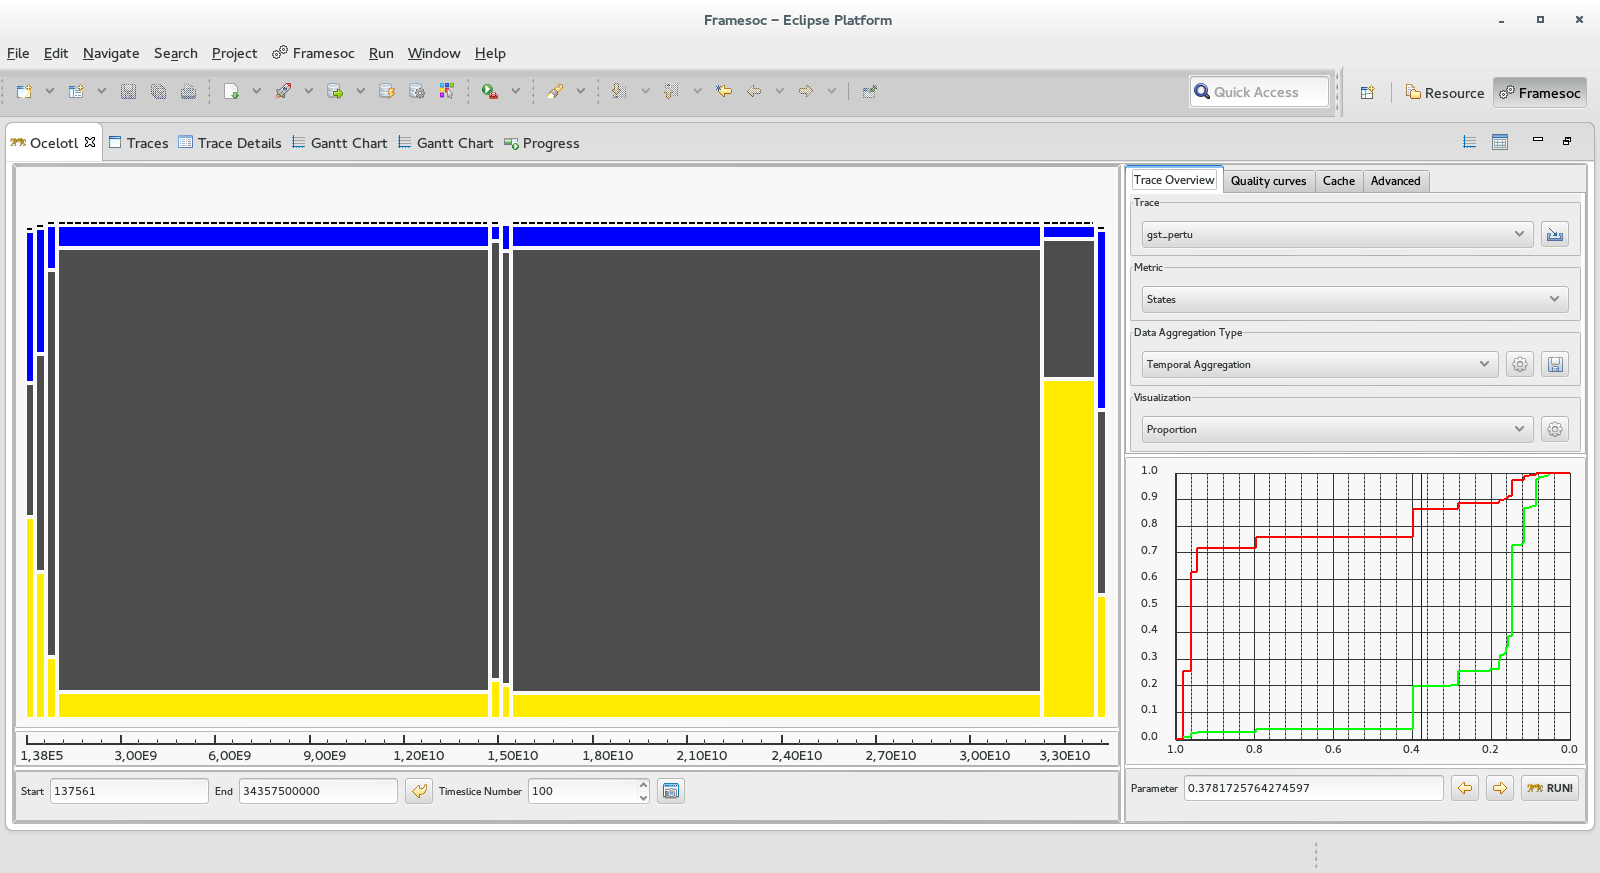
\includegraphics[width=\linewidth]{ocelotl}
    \caption[Screenshot of Ocelotl.]{
        Screenshot of Ocelotl highlighting an irregularity in a trace.\\
        Overview of the trace on the left, curves showing the impact of the $p$ parameters on the complexity of the trace on the bottom right.\\
        Image from~\cite{Dosimont14Ocelotl}.}
    \label{fig:ocelotl-overview}
\end{figure}

\gls{Ocelotl}~\cite{Dosimont14Ocelotl} is an analysis tool for \gls{Framesoc}.
This tool is particularly interesting for us as it is provide an aggregated overview of a trace.
The idea behind \gls{Ocelotl} is that a trace with too much entities (events or event producers) is not understandable, consequently, such trace should be analyzed with a \emph{systemic approach}.
This means considering the whole trace as a system and finding a macroscopic representation of that system that contain an amount of information understandable by a human.
To do so, it uses an aggregation methodology proposed by Lamarache-Perrin~\cite{Lamarche_Perrin14Agregation} and adapted for trace analysis.
This methodology cut the trace on small slices over the two dimensions time and space (event producers).
Then it consider each meaningful partition possible, benefiting from the structure on time and space to reduce the number of possibility.
For instance merging two slices that are not continuous over time is not possible as it would not mean anything.
In addition, it uses a parameter $p<[0,1]$ that controls the trade-off between information loss and data reduction and find the optimal partition for this parameters.
Once the first visualization is generated, \gls{Ocelotl} provide the ability to explore the trace (zoom, use \gls{Framesoc} filters \ldots) and change the $p$ parameter.
The usual workflow with \gls{Ocelotl} is starting with a high $p$, where the trace is mostly aggregated, zoom on anomalies or interesting parts and increasing $p$ to understand more precisely what phenomena we are observing.
To make easy the exploration, \gls{Ocelotl} provides a small window that shows the amount of information loss and data reduction for each possible value of $p$, as shown in the bottom right of \fig{ocelotl-overview}.


\subsection{Trace Description}

As explained earlier, \gls{Moca} traces are spread on five dimensions while \gls{Framesoc} is designed for two dimensional traces (time and event producers).
Nevertheless we can use the \emph{event type} of \gls{Framesoc} to differentiate reads from writes.
Moreover, event producers are organized hierarchically, therefore we can represent two dimensions as one by using this hierarchy.
For instance if we consider that each thread is a root level event producer and embed the whole memory hierarchy, we can represent at the same time memory and threads.
Finally, as we cannot reorganize dynamically the hierarchy of event producers, another workaround consist in creating several traces with different event producer hierarchy.

We designed a \gls{Framesoc} importer for \gls{Moca} traces which produces three different traces.
The first one create an event hierarchy based on the virtual memory addresses.
The second one does the same thing but for physical addresses.
Finally, in the third one, each thread is a root event producers and embed the whole memory hierarchy.

The more event producer there are, the more partitions \gls{Ocelotl} must consider to compute the aggregation.
Yet, as \gls{Ocelotl} uses the structure of the event producer hierarchy to reduce the number of allowed partitions, we can counter balanced the huge number of event producers by creating an artificial hierarchy in the memory.
We can build a meaningful hierarchy that also adds some semantic to the trace: to do so we create a virtual \emph{Memory Root} event producer that is the parent of every event producers.
Then the first level of event producers is composed of the stacks and data structures.
All the addresses that are not in these set, are merged if they are contiguous, creating chunks of continuous addresses which are also first level event producers.
Then each level is obtained by splitting the previous one on two or three parts, until we arrive at the page level.
The pages are the leaves of this virtual memory hierarchy.

\begin{figure}[htb]
    \centering
    %!TEX encoding=UTF-8 Unicode
% Palette Dark2 3 colors
\definecolor{ColF}{HTML}{1B9E77}
\definecolor{ColV}{HTML}{D95F02}
\definecolor{ColM}{HTML}{7570B3}



\tikzset{
    % Args: BeginVal, EndVal, Size, label, Color
    pics/access/.style args={#1#2#3#4#5}{
        code={
            \draw[|-|,thick,#5] (0,0) node[pos=0,below=2pt,#5]{#1} -- (#3,0)
            node[pos=1,below=2pt,#5]{#2};
            \node[ColV][anchor=south] at (#3/2,0) {#4};
        }
    },
}
\tikzstyle{mybrace} = [decorate,decoration={brace, mirror,amplitude=1em},thick]

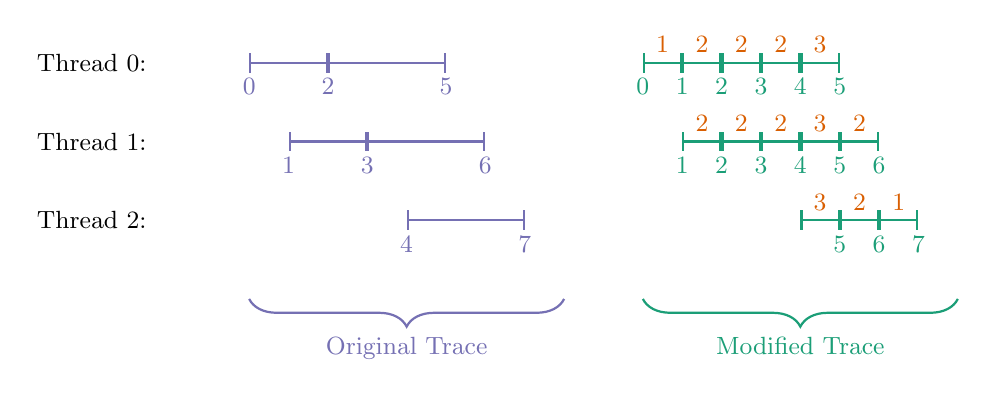
\begin{tikzpicture}[font=\small]
    \node at (-2,0) {Thread 0:};
    \node at (-2,-1) {Thread 1:};
    \node at (-2,-2) {Thread 2:};

    \draw[mybrace,ColM] (0,-3) -- (4,-3) node[pos=.5,below=1em] {Original Trace};
    \draw[mybrace,ColF] (5,-3) -- (9,-3) node[pos=.5,below=1em] {Modified Trace};

    % Moca trace
    \pic at (0,0)       {access={0}{2}{1}{}{ColM}};
    \pic at (1,0)       {access={ }{5}{1.5}{}{ColM}};

    \pic at (0.5,-1)    {access={1}{3}{1}{}{ColM}};
    \pic at (1.5,-1)    {access={ }{6}{1.5}{}{ColM}};

    \pic at (2,-2)      {access={4}{7}{1.5}{}{ColM}};

    % After parsing
    \pic at (5,0)       {access={0}{1}{.5}{1}{ColF}};
    \pic at (5.5,0)     {access={ }{2}{.5}{2}{ColF}};
    \pic at (6,0)       {access={ }{3}{.5}{2}{ColF}};
    \pic at (6.5,0)     {access={ }{4}{.5}{2}{ColF}};
    \pic at (7,0)       {access={ }{5}{.5}{3}{ColF}};

    \pic at (5.5,-1)    {access={1}{2}{.5}{2}{ColF}};
    \pic at (6,-1)      {access={ }{3}{.5}{2}{ColF}};
    \pic at (6.5,-1)    {access={ }{4}{.5}{2}{ColF}};
    \pic at (7,-1)      {access={ }{5}{.5}{3}{ColF}};
    \pic at (7.5,-1)    {access={ }{6}{.5}{2}{ColF}};

    \pic at (7,-2)      {access={ }{5}{.5}{3}{ColF}};
    \pic at (7.5,-2)    {access={ }{6}{.5}{2}{ColF}};
    \pic at (8,-2)      {access={ }{7}{.5}{1}{ColF}};
\end{tikzpicture}
% vim: et si sta lbr  sw=4 ts=4 spelllang=en_us

    \caption[Sharing detection on Moca traces.]{
        Sharing detection on a Moca trace, where three threads accesses the same page over the time.\\
        Each access is represented as an interval of time.\\
        Original trace on the left, accesses are not annotated, timelines are not synchronized.\\
        Modified trace on the right: timeline are synchronized and accesses are annotated with the number of thread involved in the sharing.
    }
    \label{fig:sharing-detection}
\end{figure}

To keep the thread information in the two first traces, we pre process \gls{Moca} traces to mark each access as shared or private.
In \gls{Moca} traces, an access is timestamped by the beginning and end of the chunk to which it belongs.
Furthermore, \gls{Moca} traces are \emph{complete} at the page granularity.
Hence, we consider that an access is shared if and only if two threads accessed the same page during intersecting time lapse.
\fig{sharing-detection} show how we transform \gls{Moca} traces to add sharing information.

Each access is represented by a variable, whose value is the number of threads involved in the access.
Our traces have four types of accesses: \texttt{PrivateRead}, \texttt{PrivateWrite}, \texttt{SharedRead} and \texttt{SharedWrite}.
Finally, the \gls{CPU} on which the access occurred is store as an event parameter.

\subsection{Example}

\begin{algorithm}
    \caption{Naïve parallel matrix multiplication.}
    \label{alg:mat-par}
    \begin{algorithmic}
        \For{i=0; i<sz; i++}
            \For{j=myid(); j<sz; j+=NbThreads()}
                \For{k=0; k<sz; k++}
                    \State Res[i][j]+=A[i][k]*B[k][j]
                \EndFor
            \EndFor
        \EndFor
    \end{algorithmic}
\end{algorithm}

To illustrate these visualizations we implemented an extremely naïve parallel matrix multiplication.
In this example, a first thread does the whole initialization, then create two threads that will do the actual computations.
Furthermore, we split the work between the threads in a round robin way, the first thread computes all even columns and the second does the odd ones as described in \alg{mat-par}.

\begin{figure}[htb]
    \centering
    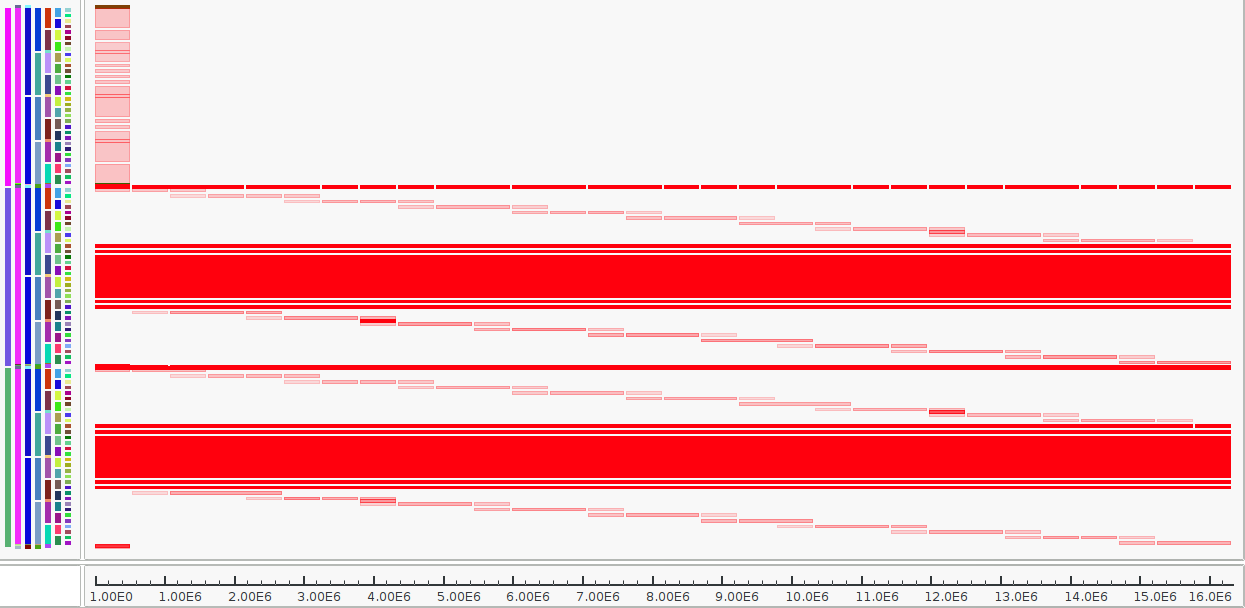
\includegraphics[width=\textwidth]{Moca-RR/multModuloThreadView.png}
    \caption{Memory-gantt view of the naïve parallel matrix multiplication.}
    \label{fig:ocelotl-th0}
\end{figure}

\fig{ocelotl-th0} is a screenshot of \gls{Ocelotl} visualization of \gls{Moca} trace, where the hierarchy starts by the threads of the application.
We can see the hierarchy on the Y-axis, starting with the three threads, each embedding the whole memory hierarchy.
The X-axis represent temporal evolution.
We call this view Memory-gantt.

From this view, we see clearly the master slave behavior of the threads.
While the two slave threads have a similar memory access pattern, the master threads do all its access at the beginning of the execution.
Moreover it seems to access all the memory at once.
We can also see that it does less access at a time as the blocks are lighter.
From this picture, we can clearly identify two phases:
\begin{enumerate}
    \item The three threads seem to use the memory, it is the initialization phase.
    \item Only two threads are awake, they follow the same access pattern: it
        is the computational phase.
\end{enumerate}

\begin{figure}[htb]
    \centering
    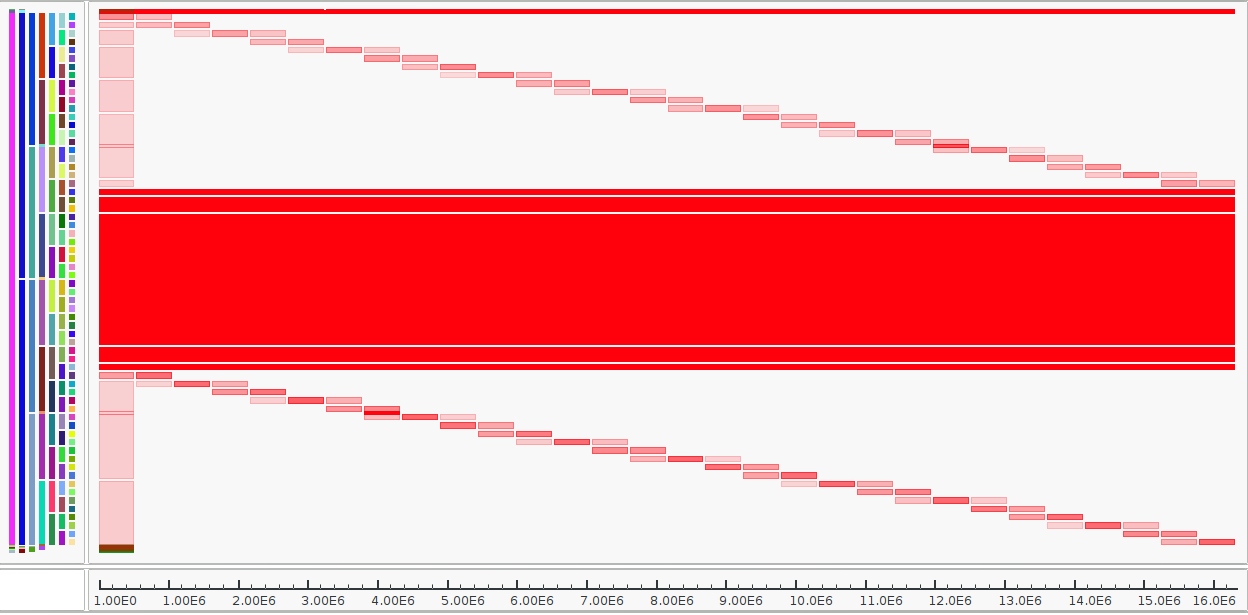
\includegraphics[width=\textwidth]{Moca-RR/multModuloCartoView.png}
    \caption{Cartography view of the naïve parallel matrix multiplication.}
    \label{fig:ocelotl-carto0}
\end{figure}

Now let's zoom on the initialisation step.
The result is shown in \fig{ocelotl-th1}.
We can clearly see that, contrary to what we thought on the last picture, during the initialisation phase, only the master thread is working.
We can identify a three diagonal patterns happening at the same time, it correspond to the matrix initialisation.
Moreover we see a few green access, while all the other are reds.
Here a red access mean that it is on a page used by several threads, while green is for private data.
Therefore we can see that the master thread also access to some private data.
Among these data, we can find a pid array used to wait the end of the slave threads.

\begin{figure}[htb]
    \centering
    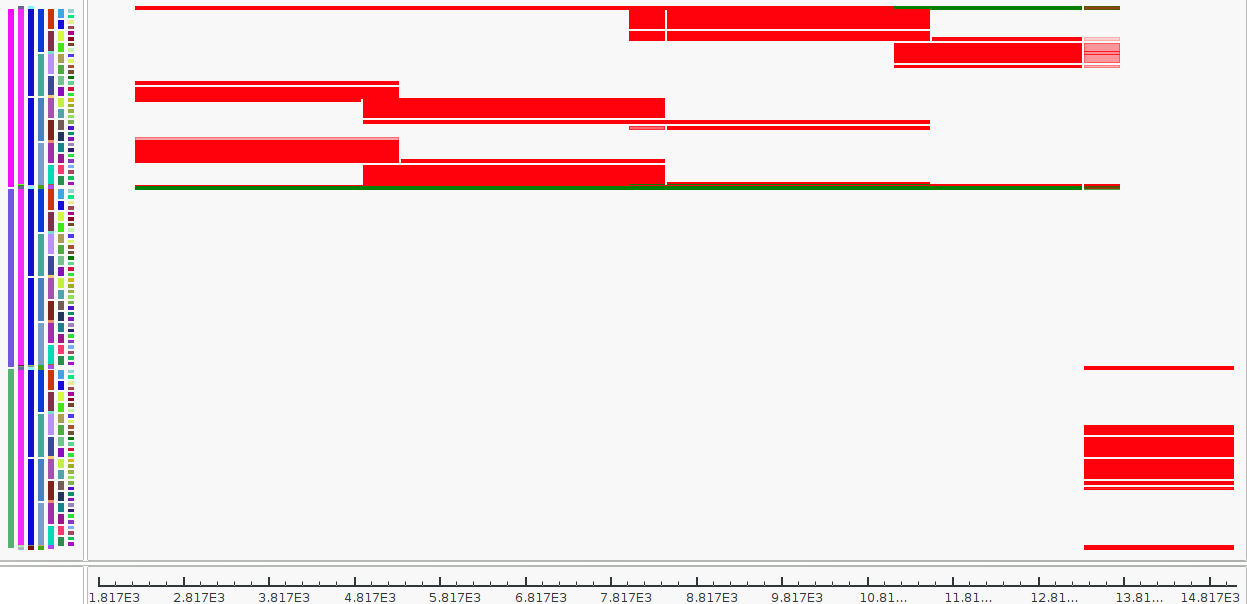
\includegraphics[width=\textwidth]{Moca-RR/multModuloThreadViewInit.png}
    \caption{Memory-gantt view of the naïve parallel matrix multiplication ,
    initialisation}
    \label{fig:ocelotl-th1}
\end{figure}

The cartography view (trace without the threads in the hierarchy) of this initialisation phase, is almost identical except that we won't be able to know which thread is responsible for the accesses.
However the global cartography view shown in \fig{ocelotl-carto0} gives more information.
In addition to the two execution phases, we can clearly identify three memory structures with different access patterns.
Those structures correspond to the matrices.
For the first and the third, we can see a regular diagonal access pattern which means that the matrix are accessed linearly, which is an efficient memory pattern.

\begin{figure}[htb]
    \centering
    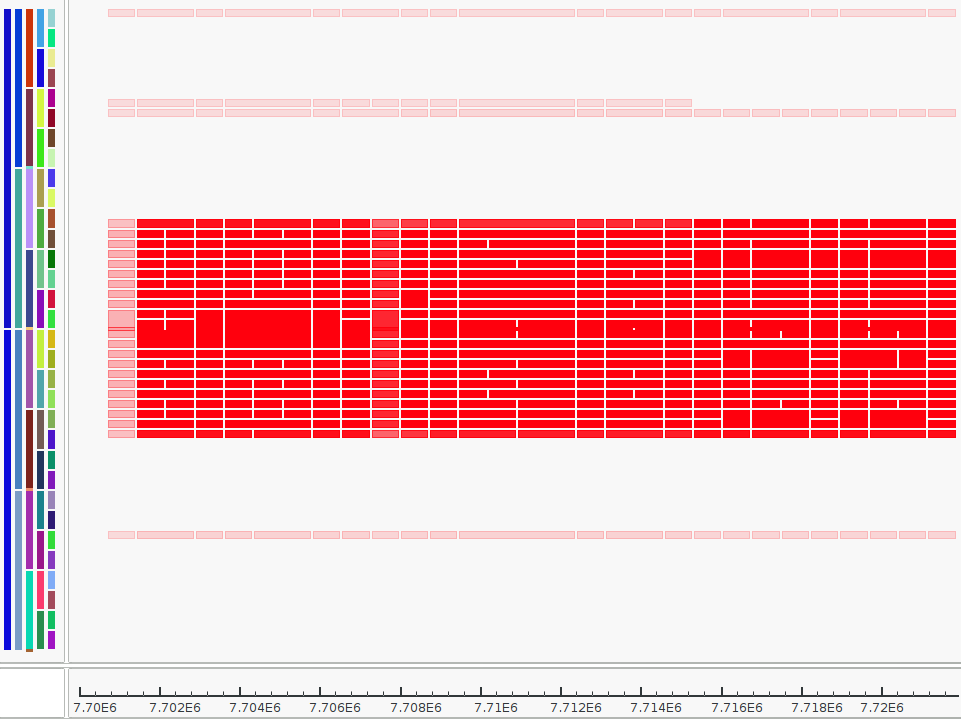
\includegraphics[width=\textwidth]{Moca-RR/multModuloCartoViewMiddle2.png}
    \caption{Cartography view of the naïve parallel matrix multiplication, computing phase.}
    \label{fig:ocelotl-Carto2}
\end{figure}

By focusing on the middle of the execution and setting the aggregation to $0$, we obtain the \fig{ocelotl-Carto2}.
We can't identify a clear pattern on the middle matrix, however, we see that at each time slots we access more a slightly different part of the matrix (the lighter a block is, the less access it contains).
The access on this matrix seems  dense and not designed to fit in a cache.
This density of accesses is coherent with the behavior describer in \alg{mat-par}
Indeed, each thread goes through all the matrix B while working on only one line of A.
Moreover the two threads works on two different columns at the same time, while the work on the same lines of A and Res.
Due to the representation of 2D matrix in \texttt{C}, each access on B is separated from $sz$ doubles.
Hence \gls{Ocelotl} groups almost everything in a huge chunks of access on all the matrices.
To improve this application, we should try to work on small blocks of B.
This is indeed the strategy used to compute efficient matrix multiplication.

\subsection{Discussion}

Although we were able to visualize all the inefficient pattern in the example described previously, we were not completely convinced of the visualization based on \gls{Ocelotl}.
Indeed, the first limitation comes from the fact that \gls{Framesoc} trace description is quite static and does not permit to change the event producers.
As a result we had to generate three traces (virtual addresses, physical addresses and by threads) to provide different visualizations.
This means that if we spot an interesting pattern in a visualization and want to look at it from another point of view, we need to reload the whole trace and  which breaks the flow of trace analysis.
Indeed \gls{Ocelotl} initial computations are slow as it needs to compare all possible partitions.
Additionally, by doing so we loose all filtering and zoom done on the previous trace.

\DB{Reformuler:}
Another limit of this approach is that it is hard to identify (name) the data structure.
Furthermore selecting only a set of data structure is slow as \gls{Framesoc} is not designed for handling as much event producers as we have with memory traces.
Finally meta data about there size or number of accesses are impossible to obtain.

To conclude, these visualization are interesting and enables identification all classic mistakes.
Yet it seems that in the end \gls{Ocelotl} tool is no well suited for memory traces.
Therefore we should try a more dynamic approach that permit to change the point of view easily.

\section{Programmatic exploration}
\label{sec:visu-second}

\begin{itemize}
    \item Exploration with R rather than full tool.
    \item Helps finding useful views
    \item R dataframes => weel design to switch point of view
    \item Work with labboks \DBm{Ref ?}
\end{itemize}

\subsection{Design}

\begin{enumerate}
    \item Parsing (csv)
    \item Retrieving mapping page => structures
    \item Creating simplified data frames
    \item Predefined plots
    \item Easily zoom  with R selection
    \item Modify plots and/or data frame
\end{enumerate}

\subsection{Results and discussion}

\begin{itemize}
    \item Small example
    \item Easy switch between views
    \item Limit: when lots of library
    \item Require that the user masters R
    \item Labook: efficient for exploring, not for reproducing same analysis on different traces
\end{itemize}

\section{Perspectives and conclusions}
\label{sec:visu-cncl}

Build user friendly trace viewer based on R analysis, using R-shiny or user friendly shell on top of R.

\subsection{Generic trace visu R}

Hypothetical tool
\begin{itemize}
    \item Goal:
        \begin{itemize}
            \item More user friendly than simple R
            \item Provide default parsing and visu
            \item Can analysis any trace
            \item Enable roll back if data frame messed up without repeating parsing
        \end{itemize}
    \item Configurations
        \begin{itemize}
            \item Define mandatory arguments (trace files)
            \item R: parsing
            \item R: Default visu
        \end{itemize}
    \item Interactions:
        \begin{itemize}
            \item Do parsing
            \item Do plots
            \item See code (parsing / plot)
            \item Apply code (possibly from models)
        \end{itemize}
    \item Data frame stack
        \begin{itemize}
            \item Every modification copy the data frame
            \item Possibility to roll back on the stack
        \end{itemize}
\end{itemize}
\DB{Figure ?}

\subsection{Automatic analysis}

\DB{Voir rapport Sebastien, sur Hopi}

\subsection{Discussions}

\begin{itemize}
    \item Still ongoing work
    \item Hard due to number of dimension
    \item Need meaningful way to zoom / aggregate
    \item Ocelotl main drawback: impossible to switch between aspects.
    \item Compromise: facility to interact with the trace, semantic of the interaction
    \item Need to put the user in the loop to filter out yet user don't know everything \ldots
    \item Possible solution: build abstraction on top of R
\end{itemize}

% vim: et si sta lbr  sw=4 ts=4 spelllang=en_us
